\documentclass[conference]{ijdc-v14}
% \documentclass[conference,15]{idcc}
%
\usepackage{graphicx}
% \usepackage[colorlinks=true,
%             urlcolor=blue,
%             citecolor=blue,
%             linkcolor=blue
%             ]{hyperref}

\usepackage{amssymb}
\usepackage{amsmath}
\usepackage{xspace}
\usepackage{apalike}
% \usepackage[
% backend=biber,
% style=alphabetic,
% maxbibnames=99,
% ]{biblatex}

\newcommand*{\Leadsto}{\ensuremath{\leadsto}\xspace}%

\newcommand{\Figref}[1]{Figure\,\ref{#1}}
\newcommand{\figref}[1]{Fig.\,\ref{#1}}

\hyphenation{data-flow}
\hyphenation{Open-Refine}
% \addbibresource{ref.bib}
% \addbibresource{newrefs.bib}

% \addbibresource{ref.bib, newrefs.bib}
%\title{\bf Improving Transparency and Reusability of Data Cleaning Recipes through Workflow Analysis}
% \title{\bf Improving Transparency and Reusability of Data Cleaning Recipes through Workflow Analysis}

\title{\bf Automatic Module Detection in Data Cleaning Workflows: \\ Enabling Transparency and Recipe Reuse} 
% \title{\bf Enabling Transparency and Reuse of Data Cleaning Recipes through Workflow Analysis and Automatic Module Detection}
%\titlerunning{Automatic Module Detection in Data Cleaning Workflows}

\author{Lan Li}
\affil{School of Information Sciences \\ University of Illinois, Urbana-Champaign}
\author{Nikolaus Parulian}
\affil{School of Information Sciences \\ University of Illinois, Urbana-Champaign}
\author{Bertram Lud\"ascher}
\affil{School of Information Sciences \\ University of Illinois, Urbana-Champaign}
\correspondence{Lan Li and Bertram Lud\"ascher. Email: \email{\{lanl2,ludaesch\}@illinois.edu}}


\newcommand{\ortoyw}{\textsf{or2yw}\xspace}
\newcommand{\orma}{\textsf{ORMA}\xspace}  % OpenRefine Model Analysis; also footprint/trace/track in Italian 
%\newcommand{\openrefine}{\textsf{OpenRefine}\xspace}
\newcommand{\openrefine}{\textrm{OpenRefine}\xspace}
\newcommand{\yw}{\textsf{YW}\xspace}
\newcommand{\yesworkflow}{\textsf{YesWorkflow}\xspace}

\newcommand{\co}[1]{\textsf{\small{#1}}}

\newcommand{\mypara}[1]{\textbf{#1.}}

\begin{document}


\maketitle

\begin{abstract}
  % Before data from multiple sources can be analyzed, data cleaning recipes usually need to be applied to improve data
  % quality. We demonstrate a Data Cleaning Conceptual Model (DC-CM) to classify operations into various types and levels
  % and analyze dependency relationships. \textbf{O}pen\textbf{R}efine \textbf{M}odel
  % \textbf{A}nalysis (\orma), a recipe
  % analyzer supported by DC-CM, is developed to provide three kinds of workflow views: table view, schema view, and
  % parallel views. We promise a more transparent and reusable data cleaning task by mapping the recipe's provenance to
  % these different granular and levels of workflow views.
  Before data from multiple sources can be analyzed, data cleaning workflows (``recipes'') usually
  need to be employed to improve data quality. We identify a number of technical problems that make
  application of FAIR principles to data cleaning recipes challenging. We then demonstrate how
  \emph{transparency} and \emph{reusability} of recipes can be improved by analyzing dataflow
  dependencies within recipes. In particular {column-level dependencies} can be used to {automatically detect independent
    subworkflows}, which then can be reused individually as data cleaning modules. We have
  prototypically implemented
  this approach as part of an ongoing project to develop open-source companion tools for \openrefine.

\bigskip

\textbf{Keywords:} Data Cleaning $\cdot$ Provenance $\cdot$ Workflow Analysis
\end{abstract}


\section{Introduction and Overview}

The FAIR guiding principles for scientific data aim to ensure that data is \emph{findable}, \emph{accessible}, \emph{interoperable}, and \emph{reusable} \cite{wilkinson_fair_2016}.
%
Metadata in general and \emph{provenance} information in particular can be used to improve
reusability of data and the reproducibility of results by increasing \emph{transparency}
\cite{nosek2015promoting,mcphillips2019reproducibility}. A major reason to provide provenance
information is to increase the trustworthiness of data by laying open its \emph{lineage}, i.e., its origins
and processing history.
% 
It is also often pointed out that data analysis % typically
consists of at least 80\% ``wrangling and cleaning'' of data, leaving only 20\% for the data
analysis proper. Not surprisingly, data cleaning ``recipes'' (or \emph{workflows}) are of central
importance in data analysis and should thus follow principles similar to FAIR data; in particular
they should be \emph{transparent} and \emph{reusable}.

Consider a user $U$ (a researcher or data curator) who wants to prepare a dataset $D_0$ for
analysis as part of a scientific study. Upon inspection she quickly realizes that $D_0$ is not ``fit
for purpose'' \cite{chapman2020developing}, i.e., its organization and data quality needs to be
improved for the intended use cases. She then employs a data cleaning tool such as
\openrefine~\cite{openrefine2020} to obtain a ``cleaner'' version that can be used for the
subsequent analyses.

An important byproduct of $U$'s interactive data cleaning process is an \emph{operation history} $H$
that can be used to describe her data cleaning workflow as a sequence of \emph{steps}
$S_1,\dots, S_n$ that transform the given $D_0$ via intermediate snapshots  into a final version
$D_n$: 

\begin{equation}
  D_0 \stackrel{S_1}{\leadsto} D_1 \stackrel{S_2}{\leadsto} D_2 \stackrel{S_3}{\leadsto} \cdots
  \stackrel{S_n}{\leadsto}  D_n ~. \label{eq-wf-history} \tag{$H$}
 \end{equation}

 This operation history $H$ can be understood as a form of \emph{provenance} information that increases
 the transparency of the data cleaning process. It contains \emph{prospective} elements at the
 \emph{workflow level}, e.g., the names of operations used, and \emph{retrospective} provenance at
 the \emph{trace level}, e.g., the concrete value changes and parameter settings used in each step.

\subsection{Technical Challenges and Approach}
% The first challenge is modeling the data cleaning provenance with $H$ to obtain different levels of granularity and abstraction of steps $S_i$. The second challenge is how to present $H$  in a form that helps others (including $U$) understand details of the data cleaning workflow that was used to obtain $D_n$. The third challenge is how to reveal the dependency relationships at the column level from details of the workflow to improve understandability.We call these challenges are the \textbf{transparency problem} for $D_n$.

The first practical challenge is how to present the history $H$ in a form that helps users (the
original workflow creator $U$, possible auditors, and other potential users) \emph{understand}
the data cleaning workflow, both at a higher, conceptual level, and at a more detailed level. We
call this the \textbf{transparency problem} for $H$.

A second challenge for $U$ is how to identify and extract from $H$ one or more \emph{reusable
  recipes} $R\subseteq H$, i.e., those elements and subworkflows of the data cleaning history that
can be reused for other datasets. We call this the recipe \textbf{reusability problem}.

There are a several other technical challenges worth mentioning: While $U$ is exploring and cleaning
a dataset, she occasionally has to backtrack and undo earlier steps to modify her workflow. To this
end, \openrefine provides an \emph{undo/redo} operation stack to support the back-and-forth of this
interactive process. She can backtrack from the current step $S_k$ to an earlier step $S_i$, inspect
the dataset at that point, and then redo the steps $S_{i+1}, \dots, S_k$. Once she decides to modify
$S_i$, however, the subsequent steps $S_{i+1}, \dots, S_k$ are typically discarded.\footnote{The
  rationale is that a change in $S_i$ may invalidate the subsequent steps $S_{i+1}, \dots, S_k$.} If
a user wants to retain some or all of these steps, they can try to work around the limitations of
the tool, e.g., by saving the steps to be re-executed and then trying to reapply them after the
modified step $S_i$.
% BL:  (\openrefine\ allows this). 
The \textbf{history update problem} is to determine which of the steps $S_{i+1}, \dots, S_k$ need to
be discarded because they no longer apply, or how to modify them so they remain applicable.
 
\textbf{Recipe migration problem.} When presented with a new but similar dataset $D'_0$, a curator
$U$ may want to reuse the parts of the history $H$ that seem applicable not just to $D_0$, but more
generally to other datasets similar to it (such as $D'_0$). Thus $U$ wants to select a {recipe}
$R\subseteq H$ for reuse, possibly revising  it as needed. Indeed $R$ is often not applicable to
$D'_0$ directly, but may have to be modified further to account for the \emph{schema
  differences} between $D_0$ and $D'_0$.

\textbf{Recipe evolution problem.} Finally, a user may want to share a recipe with a wider audience,
in the spirit of the FAIR principles. To this end, she plans to subject each candidate recipe $R_0$
to a number of tests before publishing it. Lessons learned from the tests result in a sequence
$R_0\leadsto R_1\leadsto \cdots \leadsto R_{\ell}$ of modifications to and variants of the original
recipe. The problem is how to support this evolution from $R_0$ to a publishable recipe $R_{\ell}$,
i.e., how to effectively modify, organize, and test recipes.

\textbf{Contributions.} In this paper, we focus on solving the \emph{transparency problem} and one
aspect of the \emph{reusability problem}. We employ an underlying provenance model for data cleaning
that can be used to describe data dependencies at different levels of granularity: e.g., in a
{\textbf{table view}}, we view a history $H$ as a sequence of snapshots $D_0, D_1, \dots, D_n$ in
which each new snapshot $D_{i+1}$ is derived from its predecessor $D_{i}$ via a transformation step
$S_{i+1}$.  In this way, using a coarse-grained table view, a user can get a first, high-level
overview about a data cleaning workflow. On the other hand, a finer-grained dependency analysis will
take into account the \emph{columns} that an operation reads and writes, using the input-output
\emph{signatures} of the data transformation functions that implement a step $S_i$ in the workflow.
The resulting {\textbf{schema view}} paints a more detailed and transparent picture of how the
workflow operations act on the schema, as the dataset is being transformed, step by step.  Finally,
the {\textbf{modular view}} provides another column-oriented view on the workflow: Similar to the
schema view, column-level dependencies are obtained from the recipe's dataflow graph, but now
\emph{independent subworkflows are automatically identified}, which can then form the basic building
blocks (or \emph{modules}) of reusable recipes.
%

Both the schema view and the modular view rely on a \emph{classification of operations} in order to
highlight the different kinds of effects that workflow steps have on a dataset and its
schema: % . The classification is based on the effects that operations have on a dataset:
many transformations operate on a {single} column, while others read or write {multiple} columns or
rename columns; some operations are \emph{generic} (i.e., can be applied, in principle, on any
dataset column, e.g., \co{toLower} or \co{toUpper }), while others are \emph{domain-specific}
and \emph{user-defined} (e.g., a custom mapping that fixes common misspellings over a controlled
vocabulary of city names); yet other operations convert data types (e.g., from string to number),
etc. We have prototypically implemented our approach as part of an ongoing project to develop
open-source companion tools for \openrefine \cite{orma2021}.


% The second challenge is that data cleaning task is mostly supervised task which requires human judgements and intuitions. For instance, $U$ could ``jump`` back and forth between different columns, which might reflect some intuitions and human judgement behind the recipe. The provenance information in recipe can be a resource for "reflection in action" during analysis, with which we could support collaboration between analysts, and can help trace data quality and sensemaking during the analysis process \cite{xu2015analytic}. 

% There are several contributions for this paper:
% First, we create a data cleaning conceptual model (\textbf{DC}-\textbf{CM}) to classify the operation in $H$ to various data levels: cell level, row level, column level and table level. Second, we model data cleaning recipes as \emph{workflows}, and then apply workflow and provenance analysis to workflow views. Third we enrich the workflow model by revealing the real dependency relationships at column level. Using \openrefine\ as a motivating, real-world example, we demonstrate how a set of tools can be used together to improve the transparency and reusability of data cleaning recipes.

 % workflow and provenance analysis techniques to support the use cases. Using \openrefine\ as a
 % motivating, real-world example, we demonstrate how a set of tools can be used together to improve
 % the transparency and reusability of data cleaning recipes.

\section{Data Cleaning Workflows and  \openrefine}


\begin{figure}[t]
\centering
\fbox{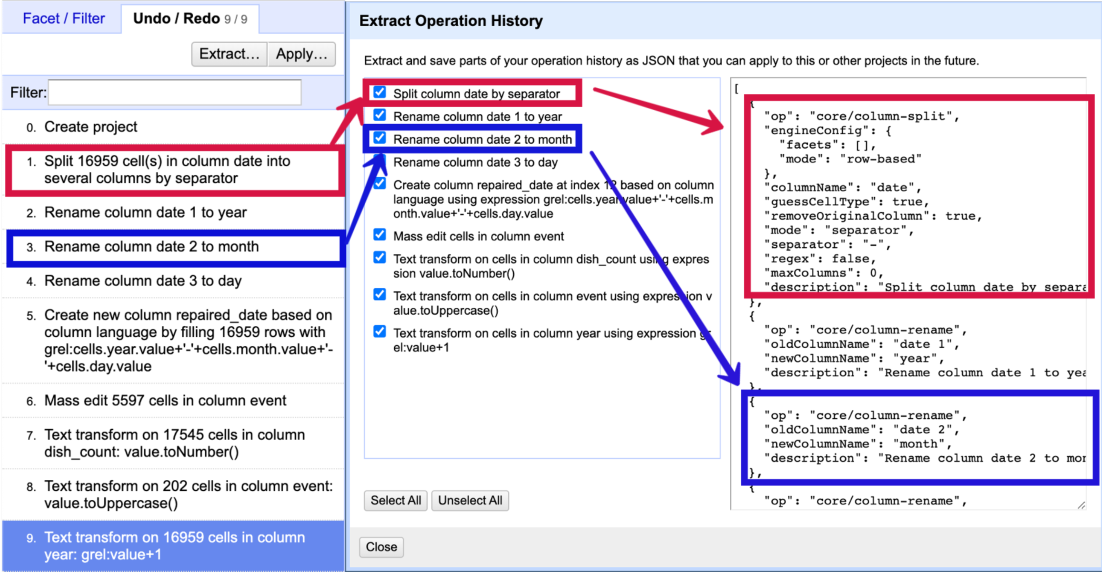
\includegraphics[width=0.95\textwidth]{idcc2021/figures/fig1-OR-history-export-crop.pdf}}
\caption{\textbf{\openrefine History and Recipe.} The {undo/redo} history $H$
(\emph{left}) shows the steps previously executed.  After clicking ``\co{Extract}'', the user can select the operations to
 be exported via a checklist (\emph{middle}). The selected recipe operations $R\subseteq H$ then appear in the JSON panel
 (\emph{right}). Steps 1 (\co{column-split}) and 3 (\co{column-rename}) are highlighted in the history, the checklist, and the JSON recipe. 
 Example taken from a recipe for the \emph{menus dataset}, crowd-sourced
 by volunteers for the New York Public Library \cite {whatsonmenu}.}
\label{fig:recipe}
\end{figure}



\openrefine\ is a popular open-source data cleaning tool that allows users to execute data
transformations in a browser-based, spreadsheet-like UI \cite{openrefine2020}.  As shown in
\Figref{fig:recipe}, the tool allows users to export an operation history $H$ as a recipe $R$ by
selecting a set of operations $R\subseteq H$. The resulting recipe can be copied and later reused
for other datasets. 

% This process $D\stackrel{H}{\leadsto}D'$ generates an operation history $H$ from which the user can select a recipe $R$ for reuse.

On the left of \Figref{fig:architecture-overview}, a typical data cleaning use case is depicted: the
user employs \openrefine\ to clean a dataset $D_0$. The process $D_0\stackrel{H}{\leadsto}D_n$
generates an operation history $H$ with $n$ steps $S_1,\dots, S_n$ from which the user can select a
recipe $R\subseteq H$ (see \figref{fig:recipe}). This recipe can then be exported in an \openrefine-specific JSON format for
later reuse. %  on another dataset. 
Since $R$ is not meant for ``human consumption'', it is rather opaque and hard to digest for users.

A first step towards improving transparency is to create a \emph{workflow model} from $R$. We 
previously developed \ortoyw\footnote{\ortoyw: an
  \textbf{O}pen\textbf{R}efine-\emph{to}-\textbf{Y}es\textbf{W}orkflow
  mapping tool \cite{or2yw}.}, which automatically generates \yw annotations from $R$. The \yw tool
uses these to create a workflow model that can be queried and visualized
\cite{mcphillips2015yesworkflow}. \yw was originally developed to allow researchers a simple way to
manually annotate their program scripts in order to reveal workflow steps and dataflow dependencies
implicit in those scripts, thereby turning an opaque script into a transparent workflow. With the
help of \ortoyw\ the user can \emph{automatically} generate \yw models from \openrefine\ recipes
(rather than manually creating them), thus providing a more {transparent workflow view} on a
previously executed sequence of data cleaning operations. For a given workflow model, the \yw tool
can generate several different views,
 e.g., a \emph{combined view} which depicts a workflow as a directed graph, linking steps via the
 data that flows between them; a \emph{process view} that emphasizes steps; and a \emph{data
   view} that highlights data derivations.

 We have since implemented \orma (\textbf{O}pen\textbf{R}efine \textbf{M}odel \textbf{A}nalysis), a
 new \openrefine companion tool that uses additional details about $H$ from \emph{project files}
 created by \openrefine when a data cleaning project is saved. The \orma prototype can then create
 ``enriched'' recipes from this information which in turn are used to create new knowledge products
 (\emph{table view}, \emph{schema view}, and \emph{modular view}) as illustrated in
 \Figref{fig:architecture-overview}.

% \ortoyw provides a potential that we could visualize the data cleaning recipe to a workflow. However, there are still several transparency problems with this workflow view. For example, operations in \openrefine are represented with the same type of data nodes in the diagram, which might bring up the ambiguity. The other concern is the recipe in \openrefine is incomplete \cite{li2019towards}. Some custom transformation like single edit is not recorded in the history $H$. This `skipping` data cleaning workflow would increase the confusion of the data cleaning task. 

\begin{figure}[t]
\centering
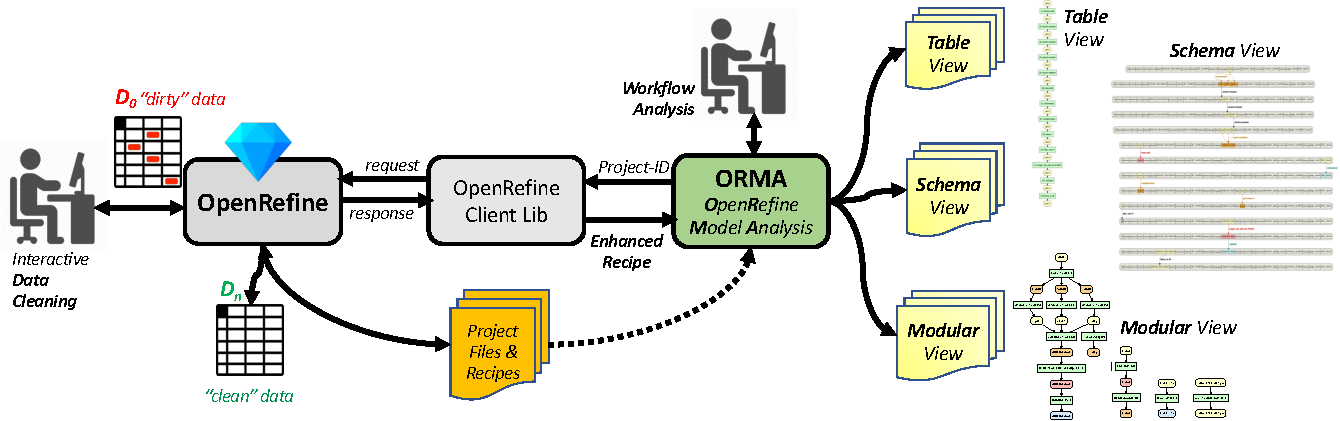
\includegraphics[width=0.95\textwidth]{figures/architecture-overview-crop.pdf}
\caption{A user cleans dataset $D_0$ with \openrefine, obtaining an
  improved version $D_n$, along with internal project files and recipes. During workflow analysis, the user
  provides \orma with a project-ID, which is then used to generate an enriched recipe (i.e., a workflow
  model). The tool then analyzes data dependencies to generate multiple views: a high-level, linear
  \emph{table view} closely corresponding to the sequential recipe, a \emph{schema view} showing
  how columns are used and updated by each step; and a \emph{modular view}, automatically
  restructuring the recipe into its independent subworkflows (\emph{modules}).}
\label{fig:architecture-overview}
\end{figure}


\section{Modeling Data Cleaning Workflows}

Before taking a closer look at some of the new views and visualizations that \orma supports,
let us first consider the underlying workflow, provenance, and data models.

\subsection{Modeling Workflows and Provenance}
\label{sec:workflows-provenance}

On the left of \Figref{fig:prov-model}, two modeling levels for data cleaning recipes are depicted:

\begin{itemize}
\item At the upper \textbf{workflow level} an operation such as ``$Y=F(X)$'' stands for any data
transformation that reads some data $X$ (e.g., from a table, a column, or a cell) and that produces
some output data $Y$.\footnote{Note that this includes the special case that $Y$ represents the
  updated version of $X$.} 
\item 
At the lower \textbf{trace level}, a concrete value $x_i\in X$ is \emph{used} by an invocation
``$y_i=F_i(x_i)$'' to \emph{generate} a result value $y_i\in Y$. 
\end{itemize}

The data cleaning recipes of \openrefine can thus be understood as workflow-level,
\emph{prospective} provenance, since they prescribe what operations should be executed (and in which
order) when the recipe is to be reused. But since recipes $R$ are obtained from operation histories
$H$, they also constitute \emph{retrospective} provenance information, since at least a partial
record of the processing history is recorded by them. 

In addition, \openrefine captures more detailed retrospective provenance in its internal
\emph{project files} (cf.\ \Figref{fig:architecture-overview}), e.g., \emph{parameter values} used
at runtime by certain operations, and \emph{deltas} that can be used to recreate any intermediate
snapshot $D_i$ when the user employs the undo/redo feature of \openrefine.

On the right of \Figref{fig:prov-model}, a simplified version of the underlying \textbf{data model} is
depicted. It shows that individual \emph{cells} are part of \emph{rows} and \emph{columns}, which in turn are part of a
data \emph{table} $D_i$. Each table is part of a table \emph{history}, i.e., a sequence of snapshots
$D_0,\dots, D_n$.
%
The power of \orma and similar tools derives from the use of a flexible underlying model that
combines prospective and retrospective information to describe data cleaning workflows, while
simultaneously supporting different data granularities (e.g., \emph{table}, \emph{column},
\emph{cell}) when describing relationships between elements. This combination allows one to create
many types of relationships between the modeling elements, beyond the simple binary relationships
(\emph{in}, \emph{out}, \emph{used}, \emph{generated-by}, and \emph{was-derived-from})
depicted in \figref{fig:prov-model}.


\subsection{Modeling Data Transformations}


The final ingredient needed by \orma to analyze data cleaning recipes as workflows is information
about {data transformations} (operations): for each data cleaning operation or function $F$, we need
to know at least its \emph{signature} $F: \bar X \to \bar Y$, i.e., the column(s)
$\bar X = X_1,\dots,X_k$ that $F$ reads (or \emph{uses}) and the column(s) $\bar Y = Y_1,\dots, Y_m$
that it writes (or \emph{generates}). In this way, by analyzing direct and indirect dependencies
between operations of a workflow, we can create different workflow views, including a modular view
which automatically detects independent subworkflows.

Consider two consecutive steps $S_i$ and $S_{i+1}$ in a workflow. A fundamental question is to
determine whether $S_{i+1}$ depends on $S_i$ (so execution must be serial) or whether $S_{i+1}$ is
in fact \emph{independent} of $S_i$ (which can be modeled using a  parallel branch in the workflow).

If the two steps are implemented by two operations $F_i: \bar X_i \to \bar Y_i$ and
$F_{i+1}: \bar X_{i+1} \to \bar Y_{i+1}$, we can test whether
$\bar Y_i \cap \bar X_{i+1} = \emptyset$. If this is the case, then the input $\bar X_{i+1}$ of
$S_{i+1}$ does not make use of any output $\bar Y_i$ of $S_i$, and we can say that $S_{i+1}$ is
{independent} of $S_i$.  In this way, a data cleaning recipe can be modeled as a workflow graph
consisting of \emph{data nodes} that represent schemas or columns, and \emph{transformation nodes}
that represent the steps (data cleaning operations) of the workflow. 


\begin{figure}[t]
\centering
~\hfill 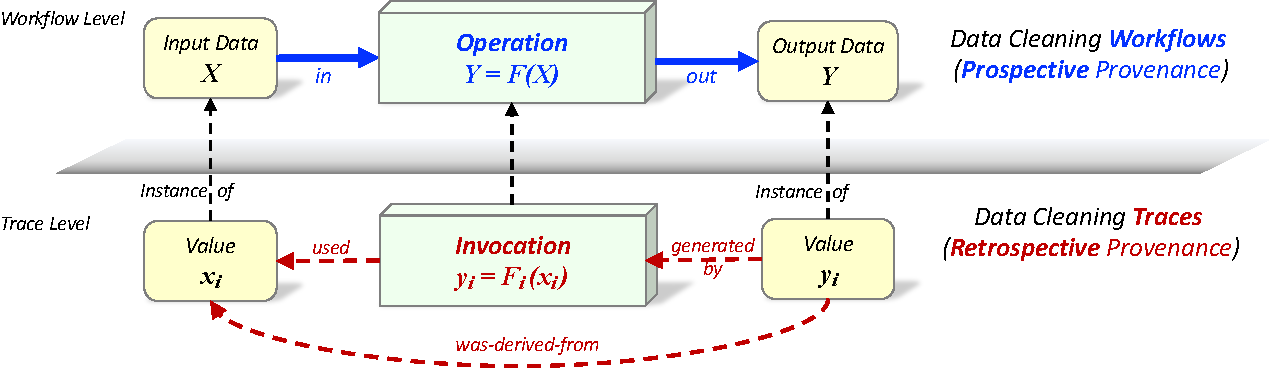
\includegraphics[width=0.75\textwidth]{figures/hybrid-prov-crop.pdf}
\hfill 
\hfill 
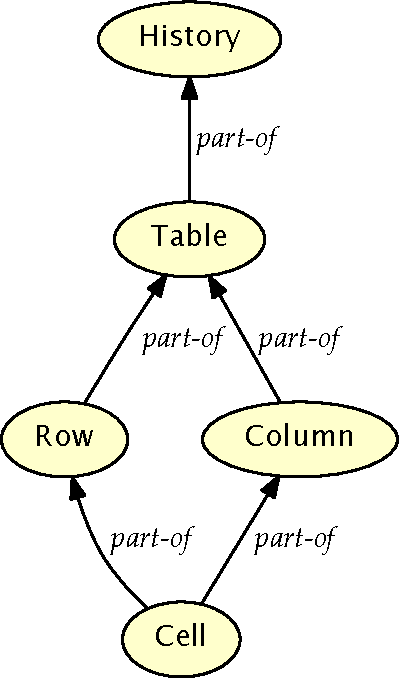
\includegraphics[width=0.15\textwidth]{idcc2021/figures/or-data-cm-crop.pdf} 
\hfill
~
\caption{\textbf{Workflows, Traces, and  Data Granularity.} 
A data cleaning recipe (\emph{workflow}) consists of data transformations (\emph{operations}) of the
form ``$Y=F(X)$'', i.e., where a function is applied to an input $X$ to obtain output $Y$
(\emph{upper left}). Workflows are a form of \emph{prospective provenance}. At runtime, an
\emph{invocation} ``$y_i = F_i(x_i)$''  yields \emph{retrospective provenance}, e.g., describing that
$y_i$ \emph{was generated by} $F_i$, which in turn \emph{used} $x_i$
(\emph{lower left}). The data being processed can be modeled at different \emph{levels of
  granularity} (\emph{right}): a {cell} can be identified by the  {row} and {column} it is
part of;  {tables} consist of rows and columns, and can have a {history} (implying that rows, columns, and cells also have a history).}
\label{fig:prov-model}
\end{figure} 




% Data Cleaning Conceptual Model (DC-CM) supports how we generate different data cleaning workflow
% views from \openrefine recipe. There are three views of data cleaning workflow: table view, schema
% view, and parallel view. Each has different granular of provenance information and dependency
% definitions. Generally, there are two types of nodes in the workflow model; one is the data node,
% the other is the process node. Data node is used to represent different levels of dataset
% information. In the table view, each data node stands for dataset snapshot $D_i$. In schema view
% and parallel view, columns applied for specific operations work as a data node. Comparably,
% Process node stands for operation $Op_i$ at each step $S_i$.

% To make sure our workflow views are transparent and explainable, we will demonstrate how we link the edges between nodes by the dependency definitions among different views and how to use the taxonomy of operation types to distinguish different nodes in the following. 

% \noindent\textbf{Dependency Definition}

% \noindent In table view, we assume a concise-grained dependency analysis, that is if a process $Op_i$ reads dataset snapshot $D_i$, and then writes a new dataset snapshot $D_{i+1}$, there would be a `deriving` dependency existing between process and dataset snapshot, and a `value` dependency existing between $D_{i+1}$ and $D_i$ (See equation \ref{eq:dep-table-view}). Consecutively, every following dataset snapshot depends on the previous one. 

% \begin{align}
% \label{eq:dep-table-view}
%     \begin{split}
%     D_0 \xleftarrow{read} Op_0 \\
%     Op_0 \xrightarrow{write} D_1 \\
%     \dots \\
%     D_{n-1} \xleftarrow{read} Op_{n-1} \\
%     Op_{n-1} \xrightarrow{write} D_{n}
%     \end{split}
% \end{align}

% In schema view and parallel view, we provide a more fine-grained dependency analysis at column level. For instance, an operation $Op_i$ works on column A, $Op_i$ writes two new column $Column_{A_1}$ and $Column_{A_2}$ (See Equation \ref{eq:dep-schema-view}). 
% Here, we could guess $Op_i$ could be transformation $Column Split$. Then next operation $Op_{i+1}$ works on $Column_{A_1}$, and $Op_{i+2}$ operates on $Column_{A_2}$. There is a dependency between $Column_{A_1}$ written by $Op_{i}$ and $Column_{A_1}$ read by $Op_{i+1}$, similar with $Column_{A_1}$. Oppositely, the $Column_{A_1}$ written by $Op_{i+1}$ could be seen as independent with the $Column_{A_2}$ written by $Op_{i+2}$.

% The strength of this fine-grained dependency analysis is, we could create a new parallel branch to describe in-dependency. Otherwise, we will use the old sequential branch to express the lineage. 

% \begin{align}
% \label{eq:dep-schema-view}
%     \begin{split}
%     \dots \\
%     Column_A \xleftarrow{read} Op_i \\
%     Op_i \xrightarrow{write} Column_{A_1}, Column_{A_2} \\
%     Column_{A_1} \xleftarrow{read} Op_{i+1} \\
%     Op_{i+1} \xrightarrow{write} Column_{A_1} \\
%     Column_{A_2} \xleftarrow{read} Op_{i+2} \\
%     Op_{i+2} \xrightarrow{write} Column_{A_2} \\
%     \dots
%     \end{split}
% \end{align}





\subsection{Classifying Data Transformations}

To make graphical workflow views more informative and intuitive for the user, different shapes and
colors can be used in \orma. For example a \emph{table view} (as in
\figref{fig:linear_view} on the left) is depicted as a bipartite graph in which rounded yellow boxes represent
table snapshots $D_i$, and green boxes represent workflow steps $S_i$ that transform one snapshot to
another. For more detailed views such as the \emph{schema view} and the \emph{modular view}, it is
helpful to classify operations according to their shared properties, and then use colors (and/or
shapes) to highlight the different effects that related operations have on the data tables.

\begin{figure}[t]
\centering
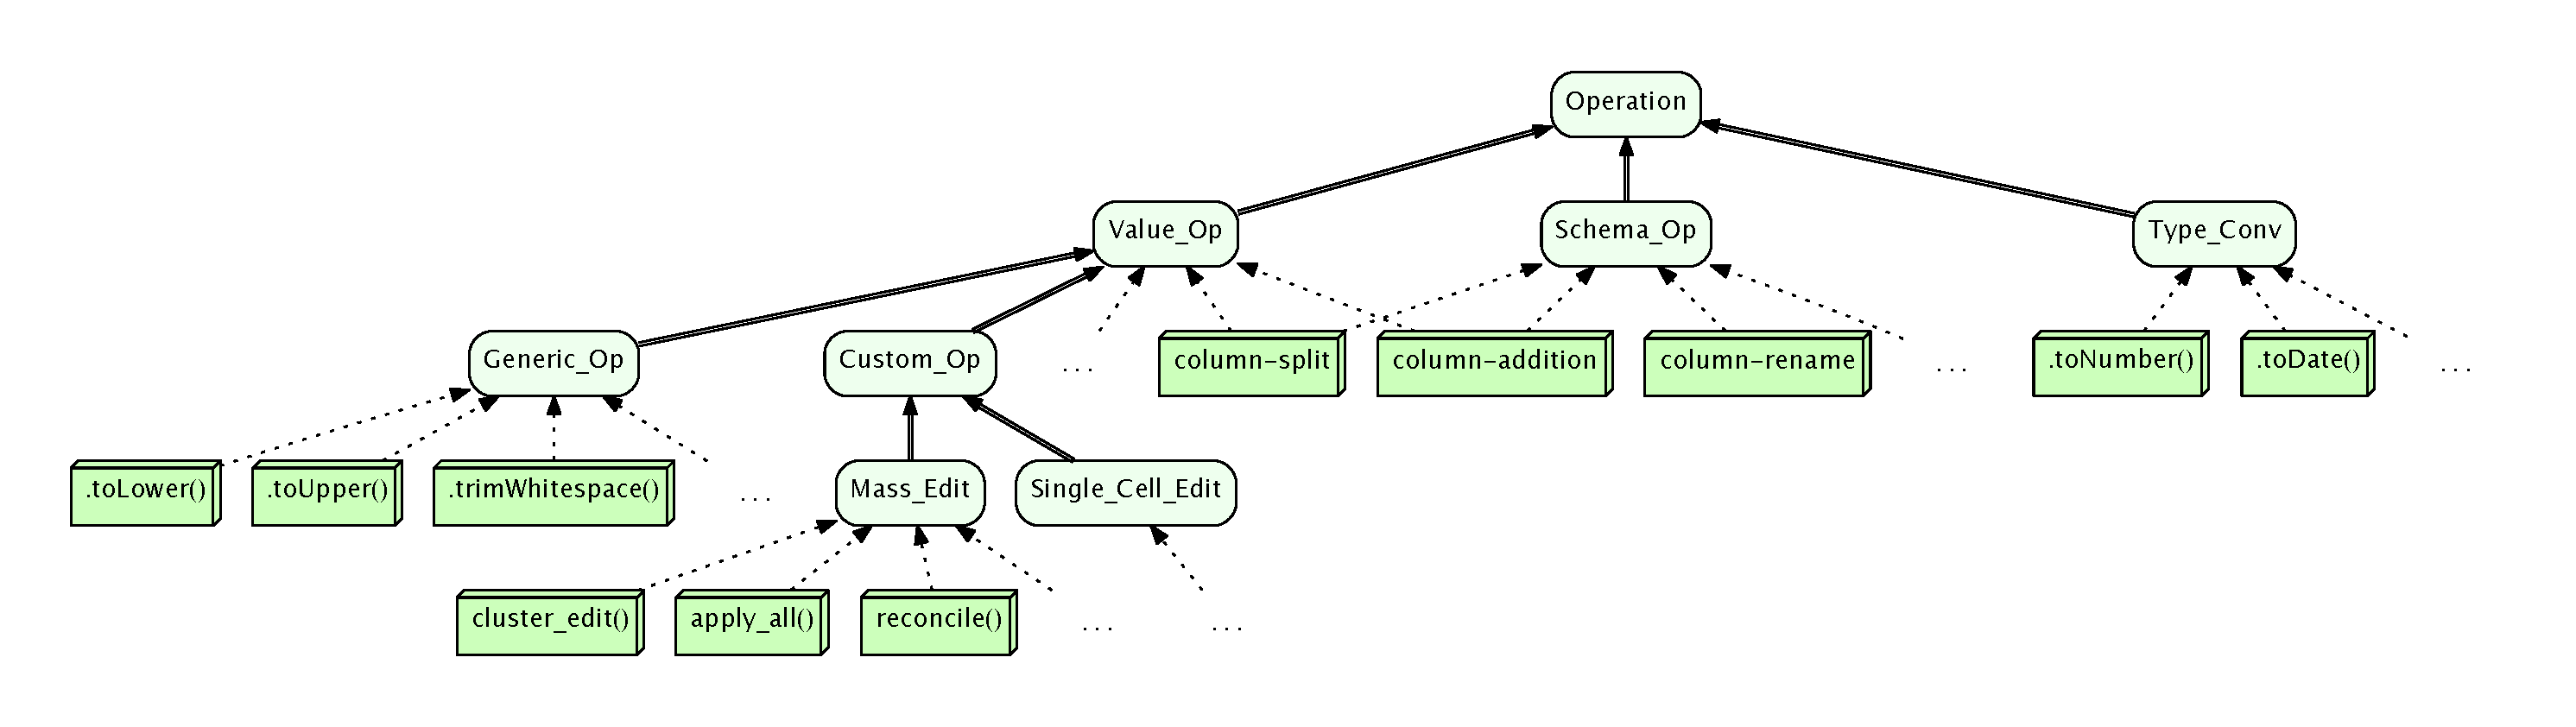
\includegraphics[width=0.98\textwidth]{idcc2021/figures/or_op_BL.pdf} 
\caption{\textbf{Classifying Operations:} \openrefine implements a range of data transformations,
  from simple, generic operations (\co{toLower()}, \co{toUpper()}, $\dots$) to powerful
  domain-specific operations requiring user interaction (e.g., for \emph{clustering},
  \emph{normalizing}, and \emph{reconciling} values), all the way to user-defined operations (e.g., using
  \emph{regular expressions}).}
\label{fig:class-operation}
\end{figure} 

\Figref{fig:class-operation} depicts a (very incomplete) view of a possible classification of the
built-in operations in \openrefine: many operations change data values (\co{Value\_Op}), some change
the data schema (\co{Schema\_Op}), and yet others the data type (\co{Type\_Conv}). Often it is also
useful to distinguish generic operations (\co{Generic\_Op}) from domain-specific operations
(\co{Custom\_Op}). While the former can be applied, in principle, on any data column, the latter may
be applicable only for certain domains of data (e.g., a mapping from common variants and mispellings
of city names to their canonical representation).  There are many other ways to organize and
classify operations, depending on the desired perspective or use of the classification. In the
current version of the \orma tool, custom operations (such as single cell edits and certain mass
edits) are prominently highlighted in red, while generic operations are highlighted in orange (cf.\
\Figref{fig:linear_view} and \Figref{fig:parallel_view}).


% Operation class hierarchy is constructing to distinguish different data nodes in the workflow,
% i.e., we could classify operations into different types through this (see
% Fig.\ref{fig:class-operation}). In this way, our workflow could be transparent and easy to
% understand.

 % There are multiple levels from top to bottom. On the top level, we classify them into value-based
 % and schema-based operations, where the prior stands for operations that change the value of the
 % cell only; the latter represents operations that change the schema of the dataset. On the next
 % level, the operations could be categorized into single-column based and multi-column based. On
 % the next lower level, they could be grouped into generic and domain-specific.  \openrefine allows
 % users to do customized transformations with their dataset. For example, the workflow of operation
 % $Cluster\_and\_Edit$ in \openrefine is, firstly, users choose appropriate clustering functions
 % and parameters to do the automatically clustering, \openrefine will return multiple `edits` which
 % is the clustering results. Users need to manually select the `edits` to avoid false positives or
 % false negatives caused by the machine learning algorithm. After the user selection, \openrefine
 % applies the selected `edits` to the column. We define this kind of operation requiring human
 % judgment as a domain-specific type. On the other hand, we see the operation $.toUppercase()$ as
 % the generic type, for these kinds of operations could be applied to any strings. Another tricky
 % transformation $.toNumber()$ is classified into type convert, belonging to single-column type.



\section{Transparency and Recipe Reuse through Workflow Views}

We are now ready to describe how \orma, our \textbf{O}pen\textbf{R}efine \textbf{M}odel
\textbf{A}nalysis tool, can be used to increase the transparency of data cleaning recipes and
facilitate their reuse.

\subsection{\orma Table View}

When using \openrefine to clean a dataset, an operation history $H$ is created, allowing the user to
extract some of the operations as a recipe $R\subseteq H$ (\Figref{fig:recipe}). Additional
provenance details can be obtained from internal project files (\Figref{fig:architecture-overview})
which \orma can then use to create different workflow views. The \textbf{table view} on the far left
in \Figref{fig:linear_view} depicts a linear workflow that corresponds one-to-one to an operation
history (similar to the one in \figref{fig:recipe}), thus making it easy for a user to see the
correspondence between the two. Through parameter switches, \orma can create different levels of
detail for table views, e.g., for a high-level overview, operation parameters can be suppressed (as
in \figref{fig:linear_view}) or alternatively, detailed parameter views can be added to table views.

\subsection{\orma Schema View}
 
The \textbf{schema view} in \Figref{fig:linear_view} is arguably more transparent than the table
view: it stills shows the sequential (linear) nature of the table view, but it also reveals which
columns are read and rewritten (updated or created anew) by each transformation step. Arrows are
used to indicate column-level dependencies between steps; arrow labels indicate the names of
operations; and colors are used to highlight the different nature of operations: columns updated
through custom operations are shown in red (possibly requiring the most attention), generic
operations in orange, and type conversions in (light) blue. Dashed arrows indicate user
interactions in the \openrefine UI, e.g., when a user ``stars'' (flags) rows, or when she is
reordering columns (e.g., \co{physical\_description: move to column \#5}).


% The \emph{table view} outputs table-level changes during data cleaning procedure (see left at
% Fig.\ref{fig:linear_view}). The table view is in a linear structure, where every current step
% depends on the prior one and all following steps derived from the previous steps. This view shows us
% an overview of data cleaning steps in the original step order from the recipe, presenting dataset
% snapshot in a concise data node. In the process node, we could check the applied operation names.


% \emph{Schema view} outputs schema-level changes after each data cleaning step (see right at
% Fig.\ref{fig:linear_view}). From top to bottom, it illustrates the sequential order from the
% recipe. Compared with the table view using one `black-box` presenting dataset snapshot, schema
% view is trying to open this `black-box` by using a transparent table composed of all columns to
% represent one dataset snapshot. We could see the column's physical position and how the number of
% columns changes at each step. Schema view also uses edges between columns to advance the real
% dependencies. Schema view presents users with a dynamic data cleaning workflow that is more
% transparent and brings up more richness of the provenance information.

% The other enhanced part for schema view is we use various colors to express different types of
% transformations according to operation class hierarchy (see Fig.\ref{fig:class-operation}). The
% more difference of the color between the input node and output code, the more attention users need
% to pay when they are using this operation. We also enrich the workflow by inviting the missing
% provenance information in the recipe. In this schema view, we extract column and row information
% from operation $single edit$. The red color is used here to emphasize this operation is
% domain-specific, by which users need to do it carefully. For the type convert operation like
% $.toNumber()$, we use green to show this operation's huge influence.

\begin{figure}[t]
  \centering
{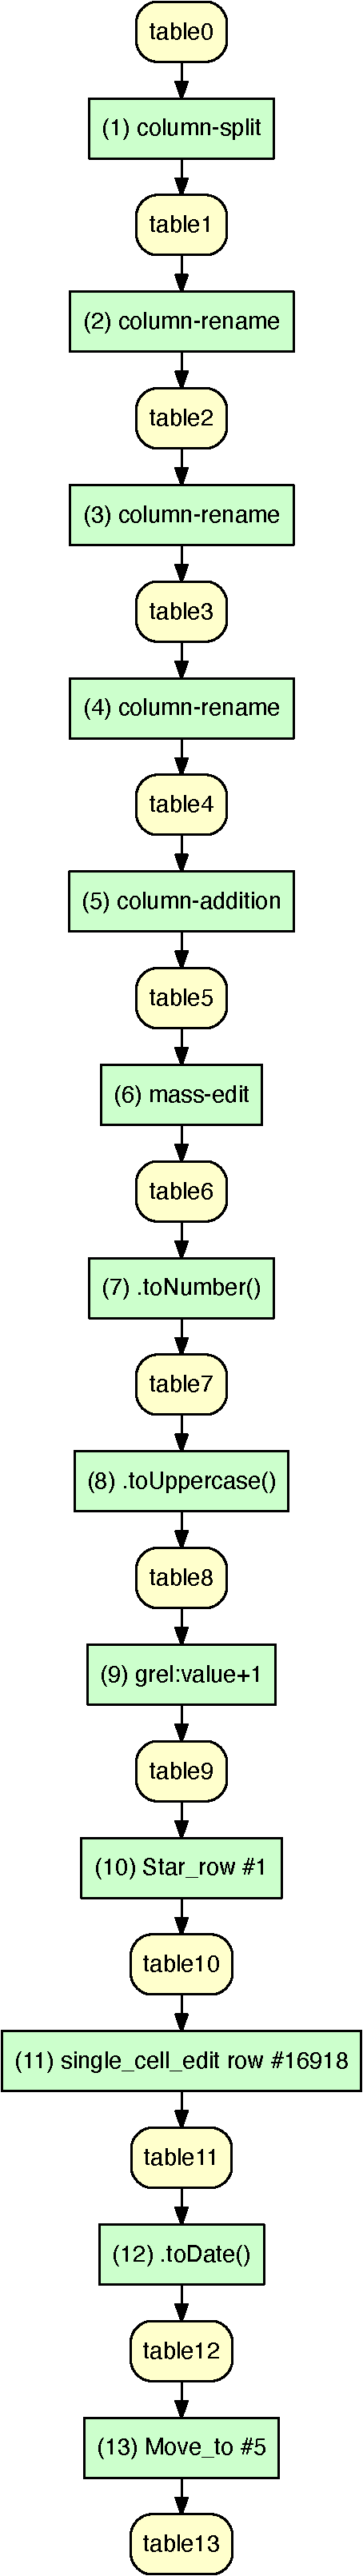
\includegraphics[height=0.4\textheight]{idcc2021/figures/table_view-crop.pdf}}
\hfill
{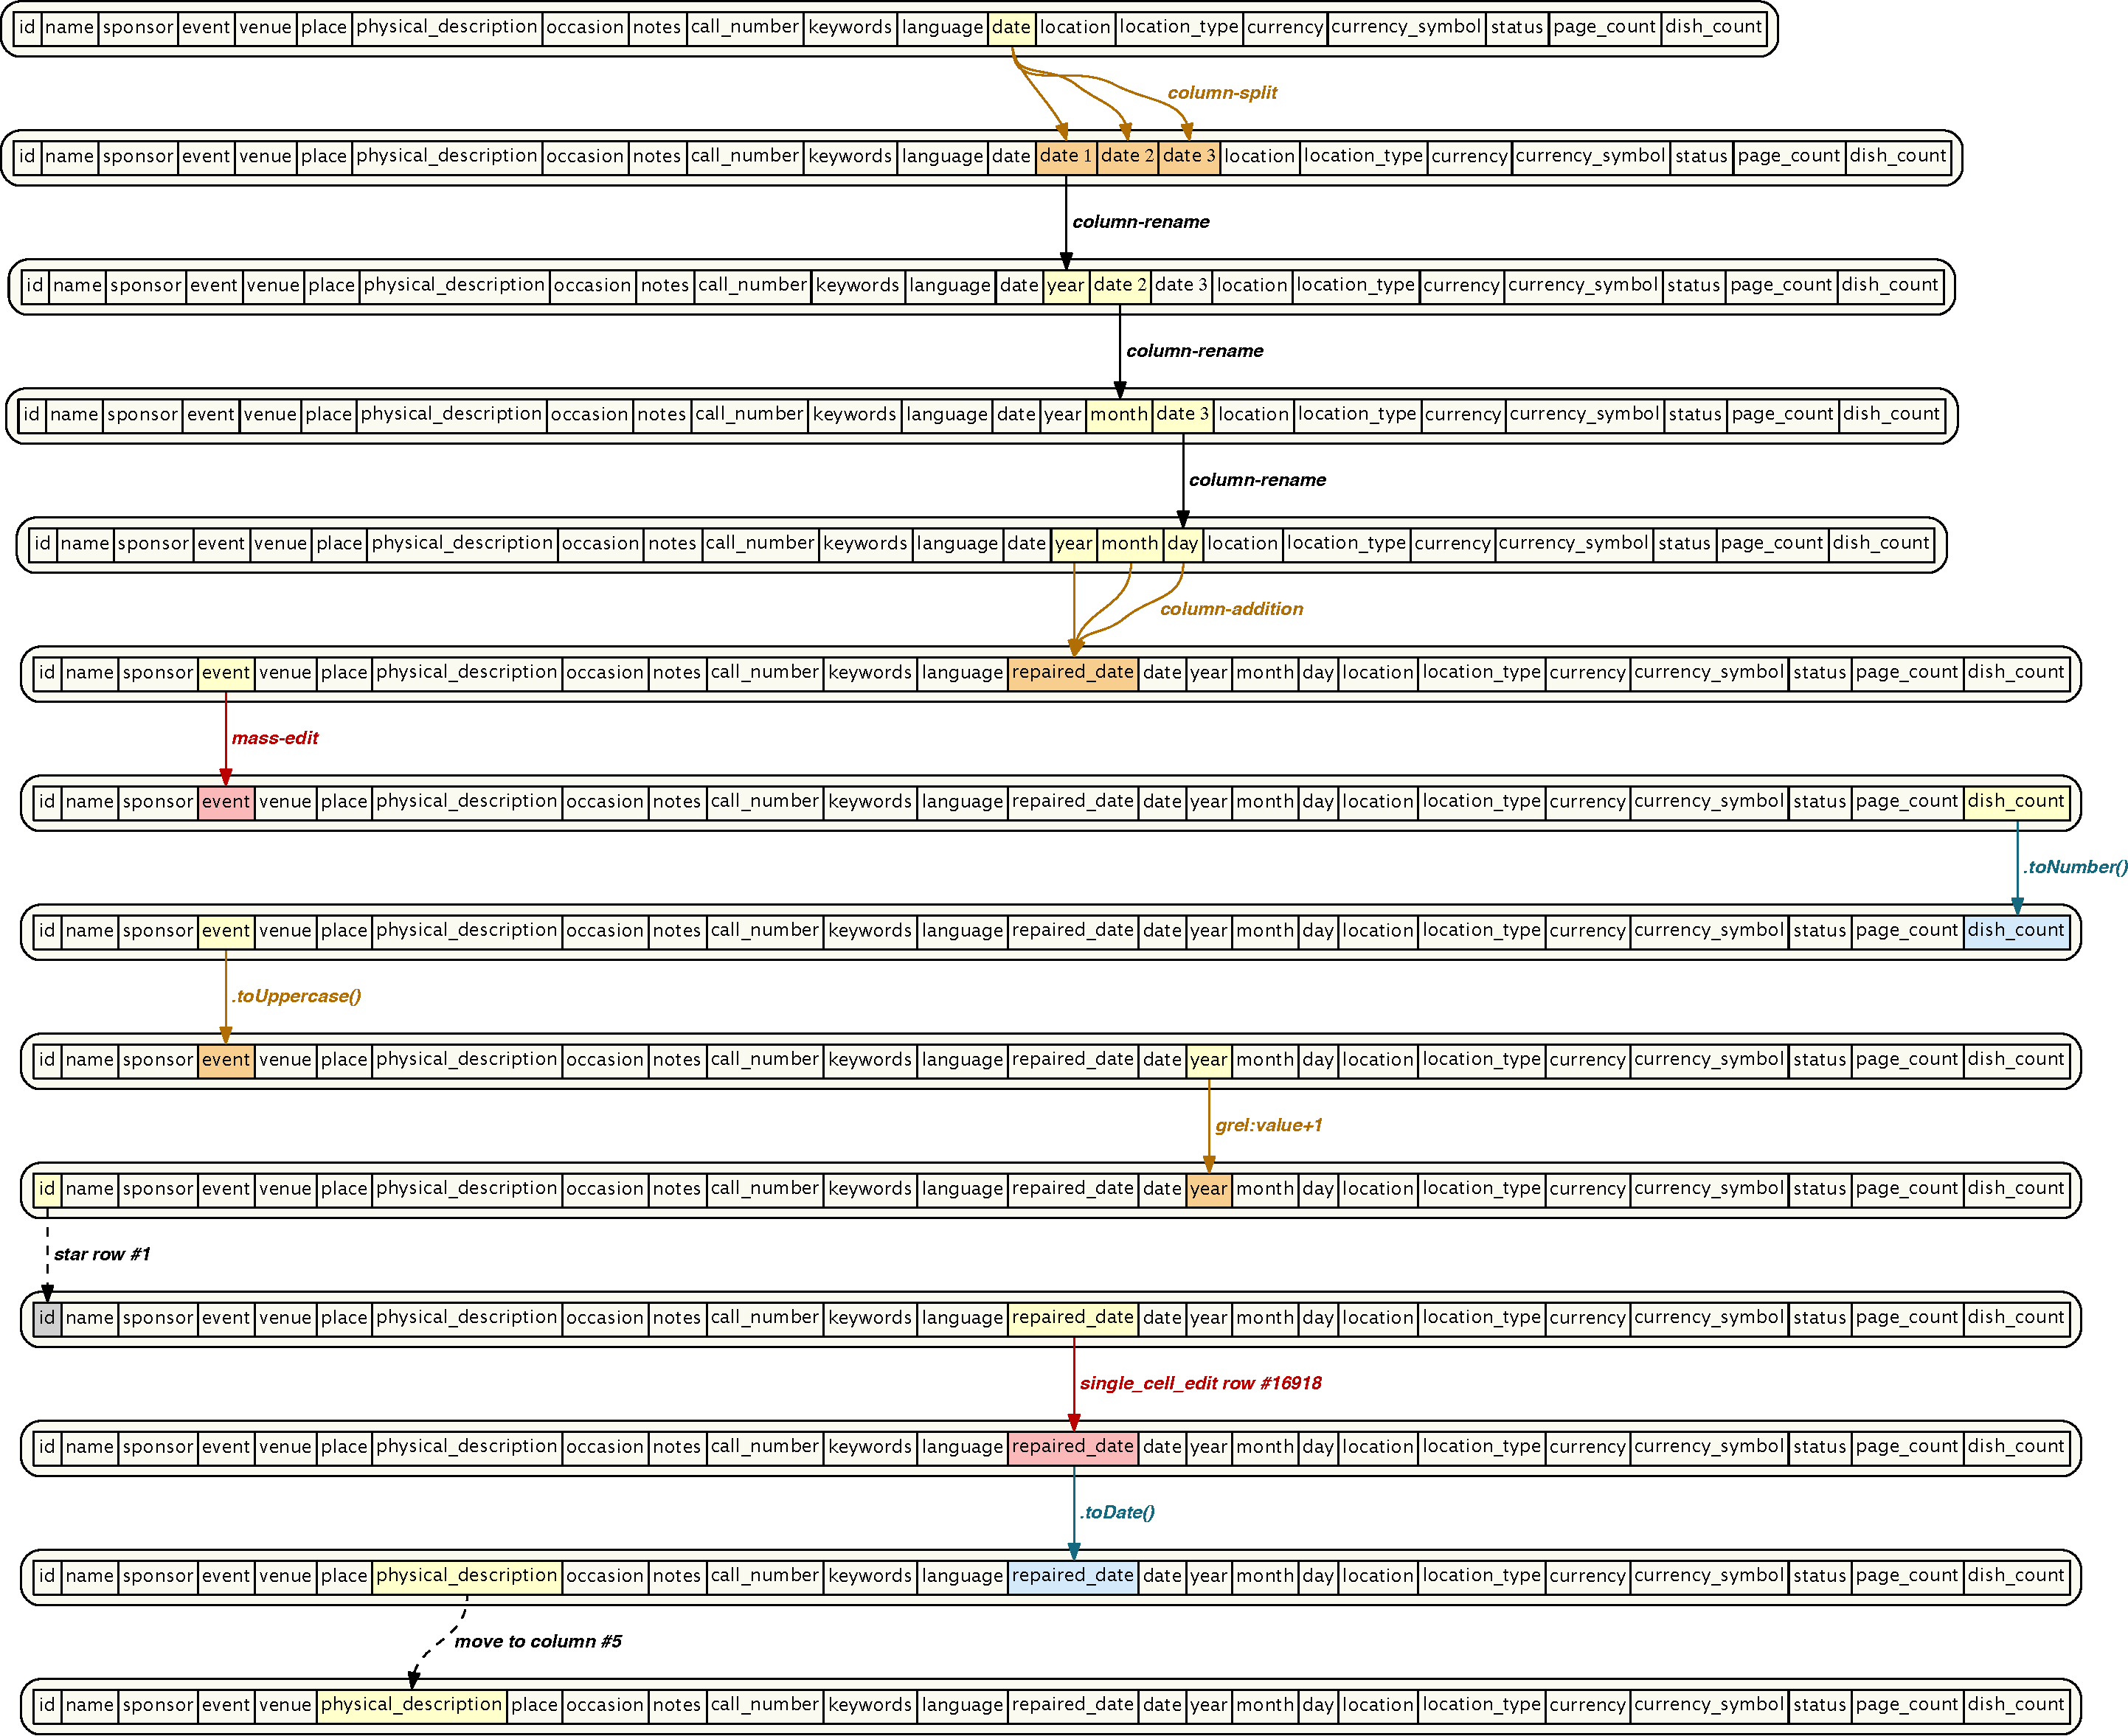
\includegraphics[height=0.4\textheight]{idcc2021/figures/schema_view-crop.pdf}} 
\caption{\textbf{Table View vs Schema View.} In the \textbf{table view} (\emph{left}) individual
  columns are not shown, and every snapshot $\mathsf{table}_{i+1}$ depends on its immediate
  predecessor $\mathsf{table}_i$. In the \textbf{schema view} (\emph{center, right}) a summary of
  changes to the schema and column-level operations is depicted: The user first worked on several
  \textsf{date} columns, then the \textsf{event} column (and other columns) before returning again
  to some specific edits on the \textsf{repaired\_date} column. Columns are colored according to the
  type of operation that affected the column.}
    \label{fig:linear_view}
\end{figure}


% The various types of information in the \emph{schema view} can be used to tackle the challenges
% identified in the introduction:
 
%  \noindent By collecting and listing all the status of schema information, we could see how a dataset is processed from a table-level view. 
 
 % \noindent Through schema analysis, we could reveal the linkage information for each data cleaning step.
 
The schema view in \Figref{fig:linear_view} also provides additional insights, e.g., it reveals that
the data curator was ``jumping around'' between different columns when cleaning the original
dataset: while the first operations (near the top and middle of the evolving schema) operate on the
\co{date} column and its derivative columns, two subsequent changes are then executed on the
\co{event} column (with an additional ``interruption'' by an operation on \co{dish\_count}). Only
near the end of the workflow does attention return to the \co{repaired\_date} column that had been
created in earlier steps.

% \noindent For additional transparency, the \emph{schema view} displays schema evolution according
% to the original sequence number, documenting how the users ``jumped'' between different columns
% while cleaning the original dataset. We could conclude their sensemaking and pattern during this
% data cleaning task in future work.
 
% \noindent This \emph{schema view} illustrates the data cleaning task efficiency and coverage by
% showing how many targeting columns are cleaned. We could do a quantitative analysis based on this
% view in future work.
 

% The resulting recipes are easier to understand and thus more suitable for migration and sharing by
% modularizing recipes and reordering the steps within recipes. Similarly, the dependency information
% is vital to address the transparency problem, as it allows the system to determine which operations
% are independent of each other. In the next chapter, we will talk about the parallel view, which
% provides more straightforward dependency relationships at the column level.

 
 


\subsection{\orma Modular View}

\Figref{fig:parallel_view} again shows a table view on the far left (for orientation and comparison)
and an automatically created \textbf{modular view} in the center, right.  Upon close inspection of
the schema view in \Figref{fig:linear_view}, one can already guess at least some elements of the
subworkflow structure exposed by the modular view. As in the schema view, the modular view depicted
in \Figref{fig:parallel_view} uses different colors to indicate the nature or type of the operations
involved (e.g., generic, custom, type conversion). \orma automatically detects all independent
subworkflows (\emph{modules} ) based on the column-level dependencies obtained from recipes and the
function signatures of operations. The modular view shown in \Figref{fig:parallel_view} still
contains the original sequence numbers of workflow steps, which helps in matching steps across
alternative views of the same workflow. In particular, the coarser-grained linear table view could
be constructed from the modular view (but not vice versa).  Modular subworkflows as the ones shown
here can be used as reusable building blocks for composing larger data cleaning recipes from a
library of independent modules. Different levels of transparency and ``verbosity'' can be chosen for
the different views supported by \orma: e.g., detailed parameter values can be included in the
views, along with other derived information (e.g., how many canonical names are part of a
\co{mass-edit} and how many variant spellings are recognized for each canonical name). 
We have omitted the display of these additional details in our figure here.

\begin{figure}[t]
  \centering
{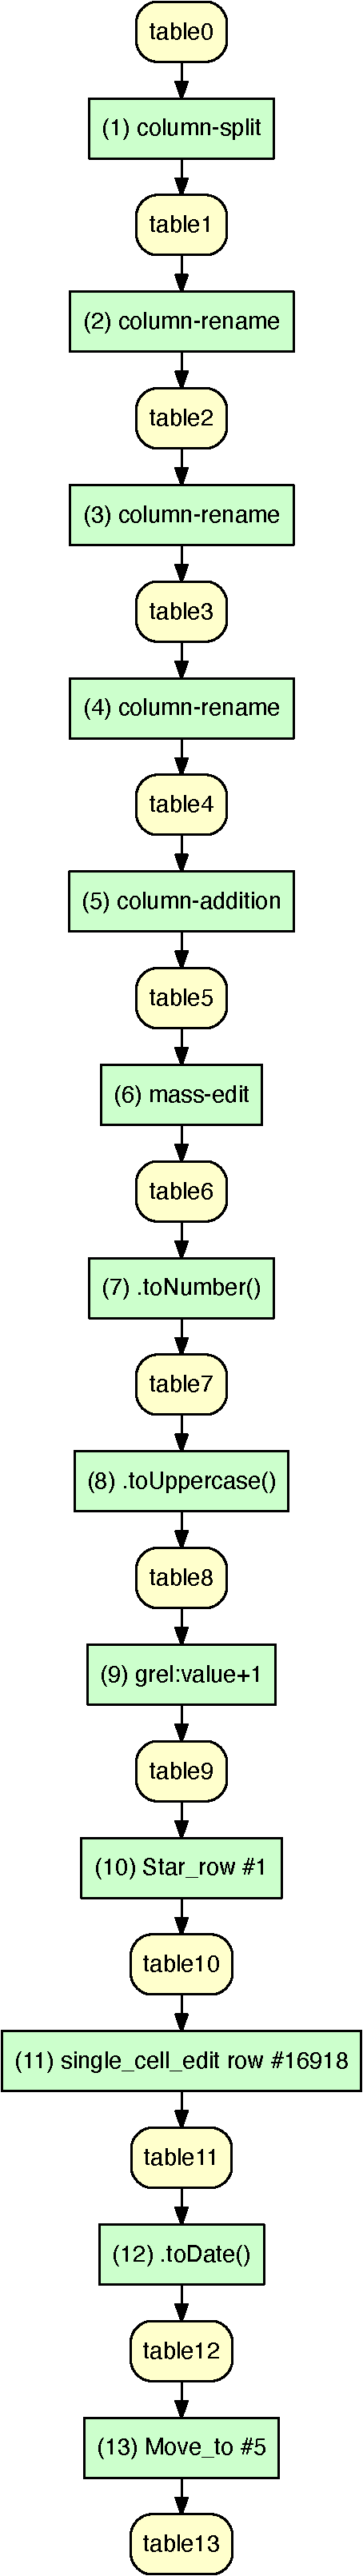
\includegraphics[height=0.33\textheight]{idcc2021/figures/table_view-crop.pdf}}
\hfill
\fbox{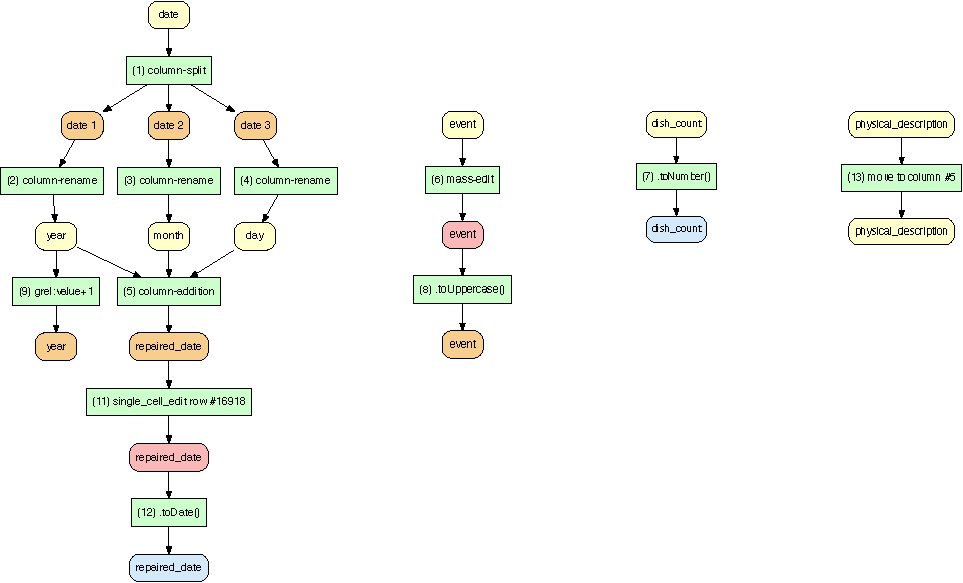
\includegraphics[width=0.79\textwidth]{idcc2021/figures/parallel-manual-layout-crop.pdf}}
\caption{\textbf{Table View vs Modular View.}  The table view on the left suggests (correctly) that
  each table snapshot depends on its predecessor via a workflow step. On the other hand, the \textbf{modular
  view} on the right highlights that the linear workflow can be decomposed into four \emph{independent}
  subworkflows (\emph{modules}), based on a finer-grained \emph{column-level} dependency
  analysis: The largest module starts from the \co{date} column, expands it by creating (and
  renaming) separate columns for \co{year}, \co{month}, and \co{day}, eventually yielding a
  \co{repaired\_date} column. The other three modules are single-column subworkflows, each working
  on their own column (\co{event}, \co{dish\_count}, and \co{physical\_description}).}  
  % It reveals that recipe $R$ consists of four \emph{independent subworkflows}, working on the
  % \emph{date}, \emph{event}, \emph{physical\_description}, and \emph{dish\_count} columns,
  % respectively. The \emph{date} subworkflow contains several \emph{parallel branches}: The date
  % column is split into three new columns, which then are renamed \emph{year}, \emph{month}, and
  % \emph{day}, respectively. A final merge step creates a new column \emph{repaired\_date}. 
    \label{fig:parallel_view}
\end{figure}



% Parallel view generates column dependency view by making column-level dependency information
% explicit in \openrefine recipe.  The way that how \ortoyw and \yw reveal the column level dependency
% information is: By ``looking inside'' the operation descriptions given in the JSON objects of a
% recipe $R$, \ortoyw can derive a \emph{signature} for each transformation in $R$: for each step
% $S\in R$ the input columns required to execute $S$ and the output columns possibly written by $S$
% are inferred. Comparably, the parallel view is more precise for it uses differences of two
% consecutive schema information to infer the column changes. With this information, parallel view
% determines whether two subsequent steps $S_i$ and $S_{i+1}$ are independent of each other: If the
% output columns of $S_i$ do not overlap with the input columns of $S_{i+1}$ and vice versa, then the
% steps commute, i.e.,
%  \begin{displaymath}
% S_i\circ S_{i+1} = S_{i+1}\circ S_i ~.    
%  \end{displaymath}

%  \noindent When the tool detects such a situation, it creates two \emph{parallel} branches in the
%  workflow, one for $S_i$ and one for $S_{i+1}$.


%  The other advanced part for our parallel view is we classify transformations into multiple levels based on the operation class hierarchy (see Fig.\ref{fig:class-operation}). Orange nodes represent generic transformation changing values only. Red nodes represent domain-specific transformation requiring human interaction. green nodes represent transformation converting data types, belonging to schema changing. Yellow nodes represent two kinds of data, including initial data snapshots and transformations which change schema only. 
%   This resulting enriched model $M^+$ and its associated {analysis view} contain details that improve the transparency and reusability of recipes: the parallel view in \figref{fig:parallel_view} reveals that $R$ consists of four independent subworkflows, one of which itself contains parallel branches. This information can be used to modularize $R$ into smaller, more reusable recipes $R_{\mathrm{date}}$, $R_{\mathrm{event}}$, and $R_{\mathrm{dish\_count}}$ which work on these individual columns only. 
 
 

\section{Conclusions}
%\input{03conclusion}

We have presented an approach to improve the transparency and reusability of data cleaning
recipes. The key idea is to model recipes as workflows over a suitable data model for describing
data cleaning processes. We have prototypically implemented an \openrefine model analyzer tool,
\orma \cite{orma2021} which can be used to create different types of workflow views, from simple
linear table views, via informative schema views, to modular views that automatically identify
independent subworkflows that facilitate reuse. In future work, we plan to tackle several other
technical challenges mentioned earlier, e.g., the history update problem or the recipe migration
problem. Another direction for future work includes the use of retrospective provenance information
to obtain even more powerful analysis methods based on hybrid models of provenance. 

% of \openrefine recipes $R$ by (i) generating a Data Cleaning Conceptual Model(DC-CM) to support
% dependency definition, and operation class taxonomy; (ii) mapping recipes to linear table view that
% helps present an overview of data cleaning procedure; (iii) using schema view to enrich the
% dependency information and operation types information in workflow view $M$ compared with the table
% view according to DC-CM; and (iv) analyzing $M$ to resolve fine-grained dependencies between data
% cleaning steps (\openrefine operations) at the column level. These three views are promising more
% transparent data cleaning workflows from syntactic perspective.

% Many directions for further research exist. In current work, we have focused on doing static recipe analysis by capturing fine-grained provenance information to ensure workflow transparency. We will do modeling and querying the enriched workflow models and make them more understandable and explainable. 

% future direction TODO
% A number of directions for further research exist. In the current work we have focused on generating workflows, i.e., \emph{prospective} provenance models \cite{mcphillips2015yesworkflow}.  We can expand the information we extract from \openrefine by ingesting the \emph{retrospective} provenance contained in project files \cite{li2019towards}. This will allow us to populate a \emph{hybrid} provenance model \cite{mcphillips2015retrospective,zhang2017revealing}, combining both prospective and retrospective provenance information. The resulting integrated model allows users to answer even more powerful provenance queries over \openrefine recipes and execution logs, further improving transparency and reusability of data cleaning recipes.


%  

% \newpage

%% ---- Bibliography ----
%
% BibTeX users should specify bibliography style 'splncs04'.
% References will then be sorted and formatted in the correct style.
%
% \bibliographystyle{../alpha-initials-big}
\bibliographystyle{apalike}
\bibliography{ref}


\end{document}

%%% Local Variables: 
%%% mode: latex 
%%% fill-column: 100
%%% TeX-master: "main"
%%% End: 
